% general
\documentclass[a4paper,12pt]{article}

% other packages
\usepackage[fleqn]{amsmath}
%\usepackage{geometry}

% graphics
\usepackage{graphicx}
\graphicspath{{./plots/}}
\usepackage[font=small,labelfont=bf]{caption}
\usepackage{float}

% hebrew
\usepackage{fontspec}
\usepackage{polyglossia}
\usepackage[utf8x]{inputenc}
%\usepackage{hebfont}
%\newfontfamily\hebrewfont[Script=Hebrew]{Miriam Mono CLM}
%\newfontfamily\hebrewfont[Script=Hebrew]{Frank Ruehl CLM}
\newfontfamily\hebrewfont[Script=Hebrew]{David CLM}
\setmainlanguage{english}
\setotherlanguage{hebrew}

% bib
\usepackage[backend=bibtex]{biblatex}
\addbibresource{bibtex/proposal.bib}

% spacing
\usepackage{setspace}
\linespread{1.25}
\setlength{\parskip}{\medskipamount}
\setlength{\parindent}{0pt}

% csv
\usepackage{csvsimple}

\begin{document}
	
	\title{PhD Proposal}
	\author{Noam Barda}
	\maketitle
	
	\section{Abstract}
	Despite reduced incidence in the developed world in recent years\cite{Koton2014,Vangen-Loenne2017}, cardiovascular disease (CVD) remains a significant cause of mortality and morbidity\cite{ODonnell2016}.
	
	Since the early 1990s, Multivariate risk models have been created to estimate patients' 10 year risk for cardiovascular events (e.g. \cite{Wilson1998,Conroy2003,DAgostino2008}). These models are used to identify patients at risk that is not due to a single factor, and are capable of exact risk quantification over time\cite{Goff2014}. Through their many variations, CVD risk models are included in different guidelines, and occupy an important place in primary prevention of CVD\cite{Graham2007,Goff2014}.
	
	The performance of risk models is highest in the population used to develop them, and is reduced on populations that are genetically or otherwise different\cite{DAgostino2001,Bastuji-Garin2002,DeFilippis2015}. Being ethnically distinct from the US and European populations used to develop existing models, CVD risk models are expected to perform sub-optimally in the Israeli population, but such external validation has not been performed yet on a population-wide scale\cite{Lovis2015}. We intend to perform such external validation on a wide sample of the Israeli population, specifically for stroke.
	
	While traditional medical risk calculators are based heavily on classic biostatistical models, mainly logistic and Cox regression, Recent advances in machine learning (specifically data availability, algorithms and computing power) allow for a new approach to medical risk modeling\cite{Obermeyer2016}. Contrary to the classic approach, emphasizing domain knowledge for the pre-specification of risk factors, novel methods instead rely on the computerized algorithms being presented with hundreds of variables and selecting the relevant ones by themselves. These variables are then used for the actual model building\cite{Weng2017}. These technologies allow a more standardized "one-size fits all" approach to risk modeling, utilizing a single comprehensive database with different outcomes\cite{Rajkomar2018}. We intend to construct such a database and utilize these algorithms to construct a novel stroke risk model to be used for this project.
	
	As use of the risk models require knowledge of test results (labs and otherwise) that patients are not generally familiar with, and the models themselves usually used to decide on treatments that require a physician to execute (e.g. statin treatment), The traditional "costumers" of medical risk models are the treating physicians, specifically those engaged in primary care. We evaluate a different approach, wherein the risk calculator is targeted directly to the patient through a sick fund's on-line website. The different variables are fed directly from the patient's electronic health record (EHR), and the patient is encouraged to view the effect of changing specific risk factors, coupled with written recommendations for risk mitigation. We will formally test the effect of such interventions in a hypothesis testing framework.
	
	\section{Hebrew Abstract}
	
	\begin{hebrew}
		למרות ירידה בהיארעותן בעשרות השנים האחרונות,\cite{Koton2014,Vangen-Loenne2017} מחלות לב וכלי דם (קרדיו-וסקולריות) עודן גורם חשוב לתחלואה ותמותה בעולם המפותח\cite{ODonnell2016}.
		
		מאז תחילת שנות ה-90 החלה יצירתם של מודלים רב-משתניים לחישוב סיכון קרדיו-וסקולרי(לדוגמה \cite{Wilson1998,Conroy2003,DAgostino2008}). מודלים אלו משמשים לזיהוי חולים בסיכון (בעיקר כשסיכון זה נובע משילוב גורמים), ומאפשרים כימות מדויק של סיכון החולה לאורך שנים רבות\cite{Goff2014}. כיום, בצורותיהן השונות, מודלים אלו כלולים בקווים המנחים של ארגונים מקצועיים רבים, ולהם מקום חשוב במניעה הראשונית של מחלות קרדיווסקולריות\cite{Graham2007,Goff2014}.
		
		ביצועיהם (ובפרט דיוקם) של מודלים אלו מיטבי כאשר משתמשים בהם באוכלוסיות שבהם פותחו, ופוחת באוכלוסיות השונות מאוכלוסיות אלו מבחינה גנטית או אחרת\cite{DAgostino2001,Bastuji-Garin2002,DeFilippis2015}. בפרט, ביצועיהם של המודלים על האוכלוסיה הישראלית, המובחנת אתנית מהאוכלוסיות האמריקאיות והאירופאיות עליהם פותחו המודלים, צפויים להיות ירודים. השערה זו טרם נבדקה על אוכלוסיה גדולה, המייצגת את האוכלוסיה הישראלית כולה\cite{Lovis2015}. אנו מתכוונים לבדוק השערה זו על מדגם נרחב של האוכלוסיה הישראלית, בהקשר של חיזוי שבץ.
		
		בעוד שמודלים קיימים לחיזוי סיכון מבוססים על שיטות ביוסטטיסטיות ותיקות, ובפרט על רגרסיה לוגיסטית ורגרסיית קוקס, חידושים מודרניים יותר בלמידה חישובית (אשר התרחשו הודות לזמינות רחבה יותר של מידע, לחידושים אלגוריתמיים ולעליה בכח המחשוב הזמין) מאפשרים גישות חדשות למידול סיכון רפואי\cite{Obermeyer2016}. בניגוד לגישה הקיימת, המבוססת על ידע תחומי לפירוט-מראש של גורמי הסיכון, גישות מודרניות מתירות לאלגוריתם החישובי, המוזן עם מאות משתנים אפשריים, לברור מביניהם את המשתנים הרלוונטיים בכחות עצמו\cite{Weng2017}. לאחר מכן, משתנים אלו משמשים לבניית המודל עצמו. טכנולוגיות אלו מאפשרות גישה יותר אחידה למידול סיכון, המשתמשת בבסיס נתונים נרחב יחיד עם תוצאים שונים\cite{Rajkomar2018}. אנו מתכוונים ליצור בסיס נתונים שכזה על מנת לבנות מודל סיכון חדש  לשבץ, אשר ישמש בעבודה זו.
		
		מאחר שהשימוש במודלים אלו דורש ידע בדבר תוצאות בדיקות (מעבדה ואחרות) שבחלקו אינו ידוע לחולים, ומאחר שהשימוש העיקרי במודלים אלו כיום הוא על מנת להחליט בנוגע לטיפולים הדורשים מעורבות רופא (כגון רישום סטטינים), ה"לקוחות" המסורתיים של מודלי חיזוי הם רופאים מטפלים, ובפרט אלו העוסקים ברפואה ראשונית. אנו נעריך גישה שונה, המציגה את מחשבוני הסיכון ישירות למטופל דרך אתר האינטרנט של קופת החולים. המשתנים השונים מוזנים למחשבון ישירות מתיקו הממוחשב של החולה, והחולה מתבקש לראות את האפקט של שינוי בגורמי הסיכון, כל זאת יחד עם המלצות כתובות בדבר הקטנת הסיכון. אנו נבדוק היעילות של התערבות זו בכלים קלאסיים של בחינת השערות.		

	\end{hebrew}
	
	
	\section{Aim of the Thesis}
	The main aim of this thesis is to implement and evaluate an intervention in the Clalit Health Services' (CHS) population meant to reduce the incidence of stroke. This intervention will be targeted directly to the Clalit's patients via an online web-based risk model that will be developed in-house as part of this project.
	
	The aforementioned goal will require three steps:
	\begin{description}
		
		\item[Model Evaluation] The intervention requires a well calibrated, discriminative risk model for stroke, capable of correctly identifying patients at high risk and correctly identifying the specific risk factor comprising their risk. As a first option, we will evaluate leading, well-known, international risk models on our patient population. This evaluation will comprise a comprehensive test of these models' performance in both their original population composition and in a shared population with the characteristics we intend to use in our intervention.
		
		\item[Model Development] As international models are often mis-calibrated when applied to new population, different than the population on which they were developed, we will develop a new model based on a modern and novel approach to developing risk models from Electronic Health Record (EHR) data. The full details of This approach will be detailed below, under "Research Methodology". This new model will be compared to existing models, and the best one chosen for the actual intervention.
		
		\item[Patient Intervention] The chosen model will be embedded within an online web-based application accessible to the Clalit's population via its online website ("Clalit Online"). The application will show the patients their risk, will allow them to interact with different variables to illustrate their effect on the risk, and will advise on ways to mitigate the risk. Following sufficient time, the intervention will be evaluated for its effect, as will be detailed under "Research Methodology".
		
		Based on these aims, we hypothesize that:
		\begin{enumerate}
			
			\item Existing risk models will have good discrimination, but poor calibration, when applied to the Israeli population. More Generally, we hypothesize that overall, their performance when validated on the Israeli population will be diminished compared to their performance as reported in the medical literature when tested on population more ethnically similar to their training population.
			
			\item That a model developed locally on the Israeli population will outperform international models.
			
			\item That using less pre-specification of risk factors, and allowing a computerized algorithm to select risk factors in an autonomous fashion, will enable detection of novel risk factors, whose inclusion in future risk models will improve their performance.
			
			\item That a direct-to-patient risk calculator, designed to present patients with their risk and allowing them ways by which to lower that risk, will result in less overall risk, improvement in risk factors and more health-seeking behavior among patients who have used the calculator.
			
		\end{enumerate}
		
	\end{description}
	
	\section{Importance and background}
	
	While the rates of cardiovascular disease in general, and stroke in particular, have declined in developed countries over the last 30 years\cite{Koton2014,Vangen-Loenne2017}, they remain significant public health problems, being the second most common cause of mortality and third most common cause of disability worldwide\cite{Lozano2012}. The statistics in Israel are similar\cite{ICDC2017}.
	
	Among diseases with such a significant public health impact, cardiovascular disease (CVD) stands out in two ways. First, its risk factors are well understood, with 90\% of its population-attributable-risk caused by 10 risk factors. It's also a very preventable disease, as these risk factors are mostly preventable\cite{Yusuf2004,ODonnell2016}.
	
	These unique characteristics have made CVD the main outcome in risk models, when such models began to enter clinical practice in the 1990s\cite{Wilson1998,NationalCholesterolEducationProgramNCEPExpertPanelonDetection2002,Conroy2003,Hippisley-Cox2007,DAgostino2008,Hippisley-Cox2008,Goff2014}. Still the most notable of said risk models is the Framingham risk model family, developed on a US population in Massachusetts, Boston\cite{Wilson1998}, and the SCORE risk model, developed in 2003 on a European population\cite{Conroy2003}.
	
	Perhaps more important that their mere existence, is that these models have made their way into widely-accepted international guidelines, with their use mandated in routine clinical care. Two examples we'll cite are the use of these risk models in deciding on Statin therapy\cite{Goff2014} and their use in deciding on anti-platelet therapy\cite{Bibbins-Domingo2016}, both for primary prevention of CVD.
	
	Naturally, risk models are developed on a specific population, whose data is available to the researchers developing the model. As patients differ in a variety of ways (both genetic and environmental), and even such basic things as lab methods and disease definitions differ in different areas, models tend to function better when used on the population on which they were developed\cite{DAgostino2001,Bastuji-Garin2002}.
	
	Recent models have tried to deal with this problem by including more ethnically varied populations\cite{DeFilippis2015} or recalibrating the model for each new population\cite{Kanis2008}, but such efforts are limited to specific risk models, and even then have only been partially successful\cite{Dagan2017}. As one specific Israeli example, this phenomenon was observed in a recent publication that illustrated significant mis-calibration for osteoporosis prediction models that are in wide clinical use and incorporated in guidelines\cite{Dagan2017}. As the probabilities generated by the model eventually help determine the proper interventions to perform, according to respective guidelines, such mis-calibration could invalidate the use of the model, making external validation an important endeavor\cite{Moons2012}.
	
	We suggest, as a first effort, to externally validate widely used risk models for the prediction of stroke risk on the Israeli population. If such models' performance is deemed unsatisfactory, this will have significant consequences for guidelines and practices based on said models.
	
	As the different risk models require knowledge of a wide variety of clinical factors, including lab results that most patients are not expected to know themselves, their use has mostly been limited to physicians. To make use of these risk models, the physician, usually the primary care physician, is required to the fill in the different covariates based on the patient's health record, communicate the results to the patient, and advise on whatever intervention is mandated to mitigate the risk. It should be said that this entire time consuming act is expected to occur in an already time-strained primary care encounter\cite{Konrad2010}.
	
	We propose an alternative to this method, whereby the risk model will be presented directly to the patient, with the different covariates extracted from the patient's electronic health record. The presentation will include an ability to view the effect of altering specific risk factors, and will include personalized recommendations for the reduction of risk based on the patient's characteristics.
	
	While CVD prediction was the bedrock for clinical risk models, they have since spread to encompass a large variety of diseases categories\cite{Kanis2008,Kansagara2011}, and have found use not only in prediction, but also in diagnosis\cite{Usher-Smith2016}. This increasingly important place taken by risk models has brought about the publication of guidelines designed to regulate and improve their creation\cite{Collins2015}. As estimating the probability for existing and future disease is a significant portion of the clinical process\cite{Moons2009}, and as this task can in large parts be automated, it seems likely that risk models will gain an increasingly important place in the medical practice.
	
	These medical risk models have generally been based on traditional biostatistical methodology (e.g. generalized linear models), and have relied heavily on the use of domain expertise in identification of relevant risk factors\cite{Weng2017}. Informally described, we could say that the model is tasked to estimate the relative weights of risk factors, themselves independently pre-identified by domain experts.
	
	In recent years the fields of machine and statistical learning have seen a tremendous rise\cite{Obermeyer2016}. this growth in machine learning, including predictive modeling, has occurred thanks to three main factors\cite{Shalev-Shwartz2014}:
	\begin{itemize}
		\item A large increase in the amount of accessible data.
		\item The development of new algorithms and methods.
		\item An increase in computation power.
	\end{itemize} 
	These new methods have several defining characteristics, including:
	\begin{itemize}
		\item The use of a wider range of algorithms, not limited to generalized linear models.
		\item Less reliance on domain expertise, in essence allowing the algorithm to both find the main risk factors and to estimate their respective weights.
		\item The need for larger sample sizes, to allow the more complex modeling to occur successfully.
	\end{itemize}
	To date, these methods have yet to gain wide-acceptance in medical practice\cite{Obermeyer2016}.
	
	Most medical risk models in wide-use were developed based on specialized cohort studies\cite{Goldstein2016}. This has the known advantages of cohort studies, most notably the accurate definition of exposures and outcomes, but is expensive and time-consuming, and by definition only allows inclusion of risk factors that were decided on in advance and measured as part of the study. On other hand, with the larger availability of EHR data, risk models developed on such data have risen in amount. These models have the known disadvantages of EHR data (first of which are the non-standardized definitions), but offer a wealth of information that in certain cases, including the case in Israel\cite{Lovis2015}, encompasses the full extent of a patient's encounters with the health system\cite{Goldstein2017}.
	
	We suggest using the unique availability of widely encompassing EHR data with large historic depth, coupled with modern statistical learning methods, to develop a generic method for generation of risk models based on the Clalit's EHR. These models will make use of most available EHR data, and will require no pre-specification of risk factors, instead allowing the algorithm to ascertain the relative importance of the different factors by itself.
	
	\section{The Novelty of the Thesis}
	
	All aforementioned aspects of the thesis contain measures of novelty to them:
	
	\begin{itemize}
		
		\item External validation of existing risk models is of utmost importance\cite{Moons2012}, as these models are used constantly as part of existing guidelines (e.g. the American Heart Association's pooled risk model and Statin treatment\cite{Goff2014}, FRAX and Osteoporosis treatment\cite{Kanis2008}). This is especially true, as previous external validation studies have at times documented significant mis-calibration\cite{Bastuji-Garin2002,Dagan2017}, that would make treatment decisions based on the models questionable.
		
		\item While development of a new risk model for the prediction of stroke in the Israeli population is important and novel by itself, we propose that the methodology by which the model will be developed, and specifically its wide applicability, requiring little human intervention and pre-processing, is by itself even more meaningful. The ability to identify risk factors and construct models for a wide variety of pathologies, some of which "unmapped" in regard to their primary risk factors, offers a promise of better understanding and more focused interventions to prevent these diseases.
		
		\item Risk-model based interventions have usually taken one of two forms: Either physician guidelines based on the risk score(e.g. \cite{Hippisley-Cox2008,DAgostino2008}); or the simple presentation of the risk model to patients, allowing them to calculate their own risk, assuming they know and have measured all their covariates(e.g. \cite{Parmar2015}). We propose a third alternative, by which a risk model is shown to the patients directly, but is "wired" into the patient's electronic health record, presenting the patient his risk based on his recorded measurements. This model is novel, and to the best of our information no previous such attempts have been made and formally evaluated. It is also particularly useful for the Israeli population, thanks to the depth on the EHR's data in Israel\cite{Lovis2015}.
		
	\end{itemize}
	
	\section{Published Work}
	
	The epidemiological characteristics of CVD in general and of stroke in particular is well understood\cite{Koton2014,Vangen-Loenne2017}, and the dominant risk factors in the population well mapped\cite{Yusuf2004,ODonnell2016}. This is true both in a the developed and in the developing world\cite{Lozano2012}. It is also true in Israel\cite{ICDC2017}.
	
	The increasingly central roles filled out by risk prediction models in medicine has been observed\cite{Moons2009}, as have the challenges of developing such models based on Electronic Health Record (EHR) data\cite{Goldstein2016,Goldstein2017}. This rapid rise in the numbers of risk prediction models has led to the writing of specific guidelines detailing methods to develop such risk models and report their results\cite{Collins2015}.
	
	Many CVD risk models have been developed in the last 30 years, most prominent of which are the Framingham\cite{Wilson1998,NationalCholesterolEducationProgramNCEPExpertPanelonDetection2002,DAgostino2008,Goff2014}, SCORE\cite{Conroy2003} and Qrisk\cite{Hippisley-Cox2007,Hippisley-Cox2008} families of models.	Two of these model families also offer a stroke-specific model\cite{Wolf1991,DAgostino1994,Hippisley-Cox2013}.
	
	Risk models have been incorporated into guidelines for the prevention, diagnosis and treatment of varying conditions. Specifically for CVD prediction, these risks help decide on cholesterol lowering treatment, anti-platelet treatment and more generally, the intensity of follow-up\cite{NationalCholesterolEducationProgramNCEPExpertPanelonDetection2002,Graham2007,Goff2014,Bibbins-Domingo2016}.
	
	Models' tendency to under-perform when the target population is changed is widely recognized\cite{DAgostino2001,Bastuji-Garin2002,DeFilippis2015} and accordingly, the importance of external validation of models prior to their use in new population is recommended\cite{Moons2012}. External validation of CVD models has been performed in several populations\cite{DAgostino2001,Bastuji-Garin2002,DeFilippis2015}, though not in the Israeli population\cite{Bitzur2015}. This is in contrary to, for example, Osteoporosis\cite{Dagan2017}.
	
	Much has been written on the advent of AI in general and machine learning in particular. In a relatively short time span, these technologies have penetrated large parts of the domains of modern life, and continue to do so in increasing force\cite{Ng2017}.
	
	That this process has been relatively slow in medicine is also widely recognized, and many efforts now exist to better incorporate such technologies in health-care\cite{Obermeyer2016}. Specifically for risk prediction models, recent literature has emerged that details attempts at the development of more generic risk models, though different than the idea proposed here both in method and in goal\cite{Rajkomar2018}.
	
	Attempts to more proactively involve patients in their own care have existed for a long time\cite{MedicineUSCommitteeonQualityofHealthCareinAmerica2001}. As AI and machine learning advance, it is only natural that these technologies will take part in such interventions. These attempts have taken varied forms: general diagnostic models based on provider statistics\cite{Aurbach2018}, smartphone apps designed to ease communications between providers and patients\cite{Sundberg2017}, wearable devices designed to encourage lifestyle change\cite{Gordon2017}, etc.
	
	More similar to this thesis are calculators presented directly to patients. These are many, and some deal directly with CVD and stroke\cite{Parmar2015}. But none of these calculators are based on locally developed models, none are able to access the patient's EHR (instead relying on him being knowledgeable about his risk factors) and non allows follow up of a patient's risk and health behavior.
	
	\section{Research Methodology}
	We will elaborate on each of the three sections in turn.
	
	\begin{description}
		
		\item[Model Evaluation] We will choose several models from the medical literature that represent the most widely known and used models for the prediction of CVD in general and stroke in particular.
		
		All covariates required for the use of each of the models will be collected from the Clalit's database. 
		\begin{itemize}
			\item Covariates that "fit" exactly (such as blood pressure, weight, etc.) will be collected as is.
			\item Covariates that are particular to a foreign country and do not exist here will be converted to the most fitting option (e.g. a foreign country's socioeconomic status scale will be converted to the Clalit's).
			\item Diagnoses will be extracted based on the Clalit's Research Institute's (CRI) deep knowledge of the structure of the database, including validation via free text.
			\item Drug treatment will be extracted based on drug dispensings, after accounting for the specific drugs and drug classes available in Israel.
		\end{itemize}
		It should be noted that studies based on the Clalit's database, and on the CRI's methods in extracting its information, have been published dozens of times (e.g. \cite{Reges2018,Dagan2017})
	
		These covariates will be collected as close as possible to the index date, but no more than three years before it. If missing at that date, we will allow collection as far as two years past the index date.
		
		Missing data will be multiply imputed using chained equations. Specifically, continuous variables will be imputed using predictive mean matching, while categorical variables will utilize logistic regression\cite{Buuren2011}. Five datasets will be imputed, with the results combined as per Rubin's law\cite{Rubin1987}.
	
		The general population for all different parts of the study is the population of patients insured by Clalit Health Services (CHS). CHS is the largest sick fund in Israel, with an insured population of 4.4 active members. Clalit is both an insurer and a provider, directly providing primary care, specialist care, lab, imaging and pharamacy services. Additionally, clalit directly operates several large hospitals. The “attrition rate” (the percentage of patients leaving the sick fund each year) stands on a low 1\%, allowing long term follow-up of patients.
		
		The data will be collected using the CHS's electronic health record (EHR). CHS has maintained a comprehensive electronic health record since the year 2000, and has continued to improve it with time. This EHR contains, among others, demographic data, medical data (including clinical covariates, lab results, imaging studies, etc.) and claims data for both services rendered as part of the mandatory health insurance and for services rendered as part of the additive insurance (“Mashlim”). This comprehensive database, combining both medical and claims data, covers large facets of a person's health.
	
		For each of the models we will generate a specific population that completely mirrors the population on which it was developed in regard to the age ranges, inclusion and exclusion criteria. This will be a "clean" external validation of the model on a different population.
		
		We will then test all three models on a common population that represents the population on which we intend to target our risk model:
		
		\begin{itemize}
			\item Ages 30-90.
			\item No past stroke event.
		\end{itemize}
	
		This will test the different models' fitness to be used for our purposes.
		
		The outcome will be defined in a similar manner for all different models. The outcome definitions will mirror those defined by a consensus committee organized by the CRI and headed by a stroke specialist. These definitions are very similar to those of the Israeli acute stroke registry\cite{ICDC2017} (active within the ICDC).
		
		Specifically for the CVD prediction models in comparison, as stroke is but a sub-category of CVD and the models are expected to be naturally mis-calibrated, we will allow the model to re-calibrate via a linear recalibration framework\cite{Houwelingen2000}.
		
		Specifically:
		
		\begin{equation*}
		\forall_i \text{LP}_i = \sum_{j=1}^{p}\beta_jx_j
		\end{equation*}
		\begin{equation*}
		\hat{y}_i = \gamma \text{LP}_i + \delta
		\end{equation*}
		
		Where $ LP_i $ is the linear predictor, $ \beta_{ij} $ is the coefficient for covariate j in patient i, $ x_{ij} $ is the covariate j in patient i, $ \hat{y} $ is the recalibrated prediction, for which $ \gamma $ is the slope and $ \delta $ the intercept.
		
		Or in words: We take the linear predictor from the original model, but allow it a new slope and intercept, thus preserving the relative importance of each covariate in the model, with the freedom to reset the global risk.
		
		For each model, we will compute the following\cite{Steyerberg2008}:
		\begin{itemize}
			\item Population table ("Table 1") for the model's specific population, including all covariates and outcomes, compared to the model's original population as published in the literature.
			\item Area under the receiver operating characteristics (AUROC) curve, or c-statistic, as a measure of discrimination.
			\item Calibration slope as a measure of calibration.
			\item Sensitivity, Specificity, PPV and NPV for the 7.5\% and 10\% risk threshold. These thresholds are chosen for their importance in existing guidelines\cite{Goff2014,Bibbins-Domingo2016}.
		\end{itemize}
		
		\item[Model Development] To develop the new model, we will generate a generic framework capable of generating models for any disease, given a fitting definition of the outcome.
		
		The framework will serve 2 consecutive tasks. The first is to choose the relevant covariates from the long list of candidate covariates supplied to it. The second is to actually build the model.
		
		It should be specifically noted that both parts carry independent significance. The covariate selection awards biological insight into the risk factors for a disease, while the model is the actual tool used for risk prediction.
		
		The covariates supplied to the first step will be: 
		\begin{itemize}
			\item Full demographic information, including age, sex, socioeconomic status, sector (arab/jew), ethnicity, etc.
			\item Clinical covariates, including blood pressure, height, weight, smoking status, etc.
			\item Lab data, including all labs performed for each patient.
			\item Chronic diagnoses, as defined by the Clalit's chronic registry\cite{Rennert2001}.
			\item Drug dispensings, including all drug dispensed to the patient.
		\end{itemize}
	
		Data will be extracted in the following manner:
		\begin{itemize}
			\item Demographic information will be collected current to the index date
			\item Clinical covariates will be collected as close as possible to the index date, but no more than 2 years before
			\item Lab data will be collected separately for the year before the index data, the year before that and the year before that.
			\item Drug dispensing data will be collected separately for the three years prior to the index date and the three years before that.
		\end{itemize}
		See the time pl
		
		Patients with a pre-existing stroke, or not of the proper age range (30-90) will be excluded.
	
		Outcomes will be collected for the 10 years past the index date with a similar definition as per part 1.
		
		The population will then be divided into a training set, a validation set and a test set.
		
		The first step will then involve applying a model to the training data that employs sparsity. That is, we will opt for models that include variable selection as a part of the fitting process. The hyperparameters for these models will be tuned using the validation set.
		
		While we intend to try several sparsity inducing models, we will describe one important such model at this point: LASSO\cite{Tibshirani2011}. other options such as gradient boosting\cite{Freund1997} and random forest\cite{Breiman2001} are similar in essence.
		
		least absolute shrinkage and selection operator (LASSO) is a variant of regression that adds a regularization term based on the $ L_1 $ norm of the coefficients to the normal loss function to be optimized. Namely, the model minimizes:
		
		\begin{equation*}
		\arg \min_w L(w) + \lambda \sum_{i}|\beta|_i
		\end{equation*}
		
		L being the likelihood function and lambda being a regularization parameter. Owing to the geometric structure of the $ L_1 $ norm, this has the effect of setting many covariates to 0, inducing sparsity. The parameter lambda is selected using cross-validation on the validation set, with predictive performance (e.g. AUROC) as the goal.
		
		The model as produced by the sparsity inducing algorithm will be compared to the existing models examined in phase I using the above mentioned performance measures. For the sake of demonstrating clinical utility, we will also compare the best model from phase I to our model for net reclassification improvement\cite{Pencina2008} and decision curves\cite{Vickers2016}.
		
		While in essence we could use the models from phase I or the model as produced by our sparsity inducing algorithm as is, the requirement of using the model in a web application, including tight memory and responsiveness constrains, forces us to fit a simpler final model.
		
		To account for this, we will take the covariates from the best model and use them construct a simple logistic regression model. This will be our final model to be used in the application.
		
		For this section, we'll strictly adhere to the TRIPOD guidelines\cite{Collins2015}.
		
		Study time-line for parts 1 and 2:
		
		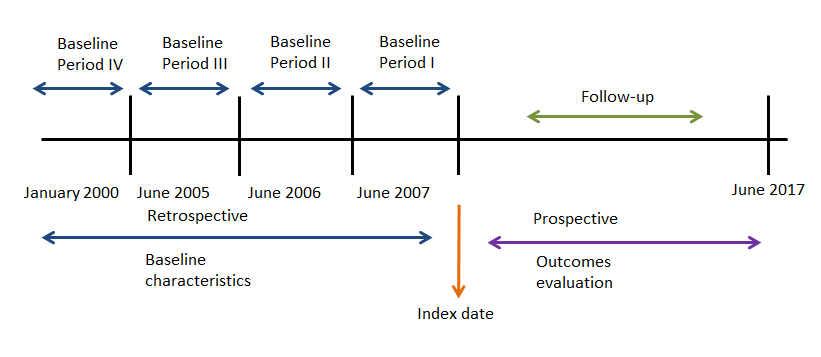
\includegraphics[width=\textwidth]{prelim-results/Panpredictor/timeline.png}
		
		\item[Patient Intervention] Once the models are deployed to the Clalit's website, we will allow several months for the accumulation of a user population and results. We will then check the three hypotheses originally stated:
		
		\begin{itemize}
			\item That users of the model improved their overall risk profile.
			\item That users of the model improved specific risk factors.
			\item That users of the model utilized more health services.
		\end{itemize}
	
		This will be tested in two comparisons:
		\begin{itemize}
			\item The first is a self controlled case series (SCCS) method, whereby we conduct a paired comparison of each patient to himself in the immediate time prior to the use of the model. This allows us to implicitly account for confounders without explicitly adjusting.
			
			\item The second is a more classic cohort design, matching the users to non-users (in a ratio as will be determined by a power analysis - DO THIS) on age, sex and overall baseline risk.
		\end{itemize}
	
		The outcomes will be determined by evaluating the risk 3 months post intervention. Health utilization will be determined by counting overall health utilization, including physician visits, hospitalization and drug dispensings. Standardization across health utilization categories will be achieved using the overall monetary cost of the patient to the insurer.
		
		Continuous outcomes will be compared using student's t-test. Categorical outcomes will be compared using the chi square goodness of fit test.
		
	\end{description}
	
	\section{Preliminary Results}
	We will present preliminary results for each of the 3 portions.

	\subsection{Part 1}

	Population Table for the Framingham Stroke Risk Score\cite{DAgostino1994} model:

	\csvautotabular[separator=pipe]{prelim-results/FSRS/T1.csv}
	
	Calibration and ROC Curves for the Framingham Stroke Risk Score model:
	
	\begin{figure}[H]
		\begin{minipage}{.45\linewidth}
			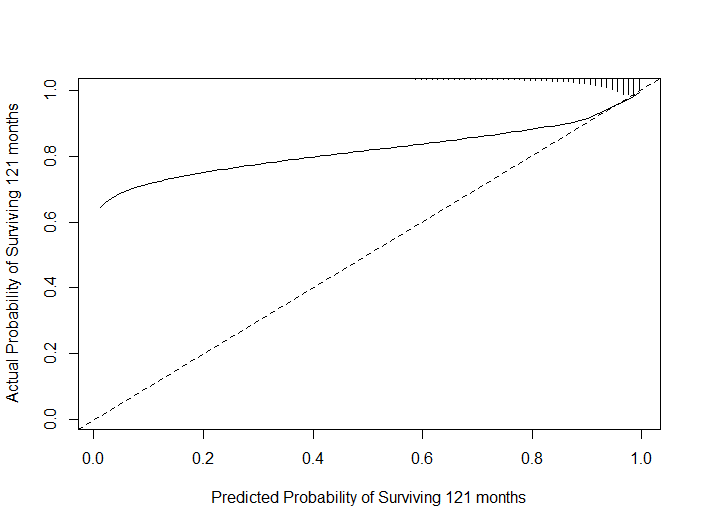
\includegraphics[width=8cm, height=8cm]{prelim-results/FSRS/FSRScal.png}
			\label{FSRS1}
		\end{minipage}
		\hspace{.01\linewidth}
		\begin{minipage}{.45\linewidth}
			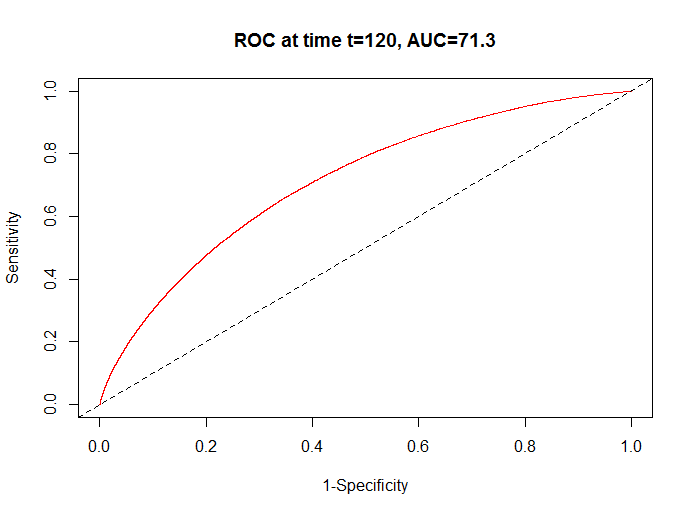
\includegraphics[width=8cm, height=8cm]{prelim-results/FSRS/FSRSdisc.png}
			\label{FSRS2}
		\end{minipage}
	\end{figure}
	
	\subsection{Part 2}
	
	Preliminary ROC curve for the Clalit model:
	
	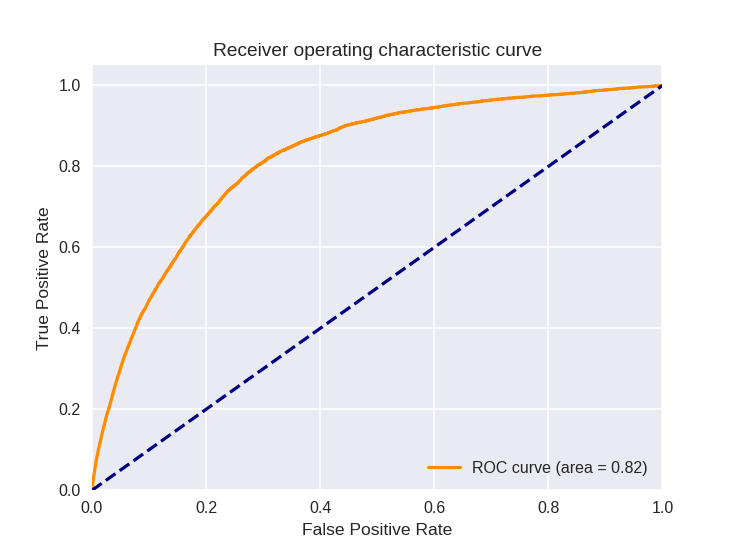
\includegraphics[width=10cm,height=8cm]{prelim-results/Panpredictor/ROCCurve.png}
	
	\subsection{Part 3}
	
	Early draft of the calculators for the Clalit's website, this specific one for chronic kidney disease. Eventually, the finalized stroke calculator will look similar.
	
	\begin{figure}[H]
		%\centering
		\begin{minipage}{.3\linewidth}
			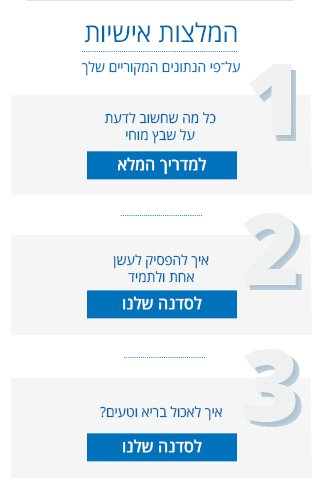
\includegraphics[width=4.5cm, height=7cm]{prelim-results/calc3}
			\label{calc3}
		\end{minipage}
		\hspace{.01\linewidth}
		\begin{minipage}{.3\linewidth}
			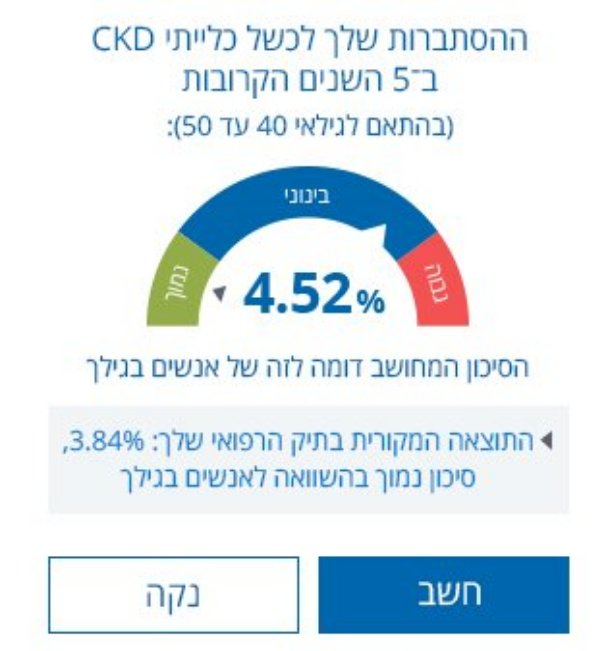
\includegraphics[width=4.5cm, height=7cm]{prelim-results/calc2b}
			\label{calc2}
		\end{minipage}
		\hspace{.01\linewidth}
		\begin{minipage}{.3\linewidth}
			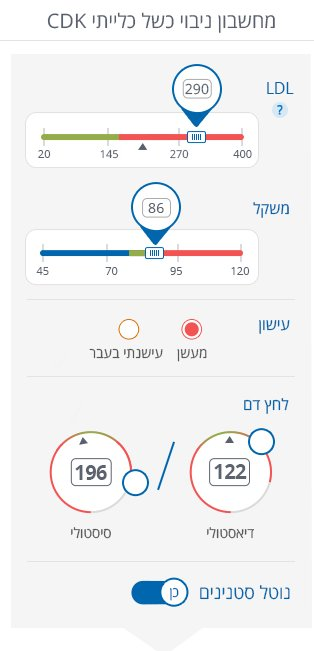
\includegraphics[width=4.5cm, height=7cm]{prelim-results/calc1}
			\label{calc1}
		\end{minipage}
	\end{figure}
	
	\section{References}
	
	%\nocite{*}
   	\printbibliography[heading=none]
	
\end{document}